\cleardoublepage
\chapter{Software}
% To do: 
% Color Scheme
% Red - Not started
% Yellow - In progress
% Blue - Done, under approval
% Green - Done and approved
\todo[inline,color=red!40]{*Chapter Introduction}
\todo[inline,color=blue!40]{*1 - Microphone}
\todo[inline,color=yellow!40]{*2 - Microcontroller}
\todo[inline,color=blue!40]{ a) Peripherals}
\todo[inline,color=blue!40]{ b) FFT implementation}
\todo[inline,color=blue!40]{ c) Fixed-Point Square Root}
\todo[inline,color=red!40]{*3 - MatLab}
%%%%%%%%%%%%%%%%%%%%%%%%%%%%%%%%%% Writing %%%%%%%%%%%%%%%%%%%%%%%%%%%%%%%%%%%
%brief acknowledgment of what pieces are part of the developed software, add in the end a section how is intended to find the liquid level
\section{Microphone}
As the first measurements will be taken recurring to a microphone, it requires a different approach to the type of interaction when compared to the future application, were will be use a different sensor for the vibration. To obtain access and record the information from the microphone and for this case in specific, since is being used the microphone from a phone, will require different pieces of software to use in the phone side and the PC, to allow the access to the second to the microphone of the first. Also, on the PC side is necessary to record the information from the microphone and store it as desire.\\
The two components for this purpose will be the use of the WOMic software as the bridge between the phone and the computer, and MATLAB to record the information from the microphone. The second software can also be used to latter process the recorded data, helping the understand of the obtained information. 
\subsection*{WOMic}
The use of the application and the microphone of the phone is simple, although the installation and the configuration requires some time. For that, is required to install the software \textit{WOMic} in both devices, this allow to use the microphone of the phone in real-time. In the phone the software is available for Android and IOS and is responsible to transmit what is captured from the microphone, in the computer the client application and a virtual device must be installed to use the microphone in the PC to perform any type of tasks, this connection can be made over USB, Bluetooth, Wi-Fi and Wi-Fi Direct.\\ 
In order to save what is captured from the microphone, the software is split in three main block with different purposes, the \textit{WOMic App} runs in the phone, samples the input of the microphone and transmit it to the computer, the \textit{WOMic Client}, runs in the PC, connect to the app in the phone, and receive the data from the microphone, which is transmitted to the \textit{WOMic Virtual Device} on which a real microphone device is simulated and provides the audio to any application or program in the PC, as illustrated in figure \ref{fig:diagramWOMIC}.\\
\begin{figure}[!htb]
    \centering
    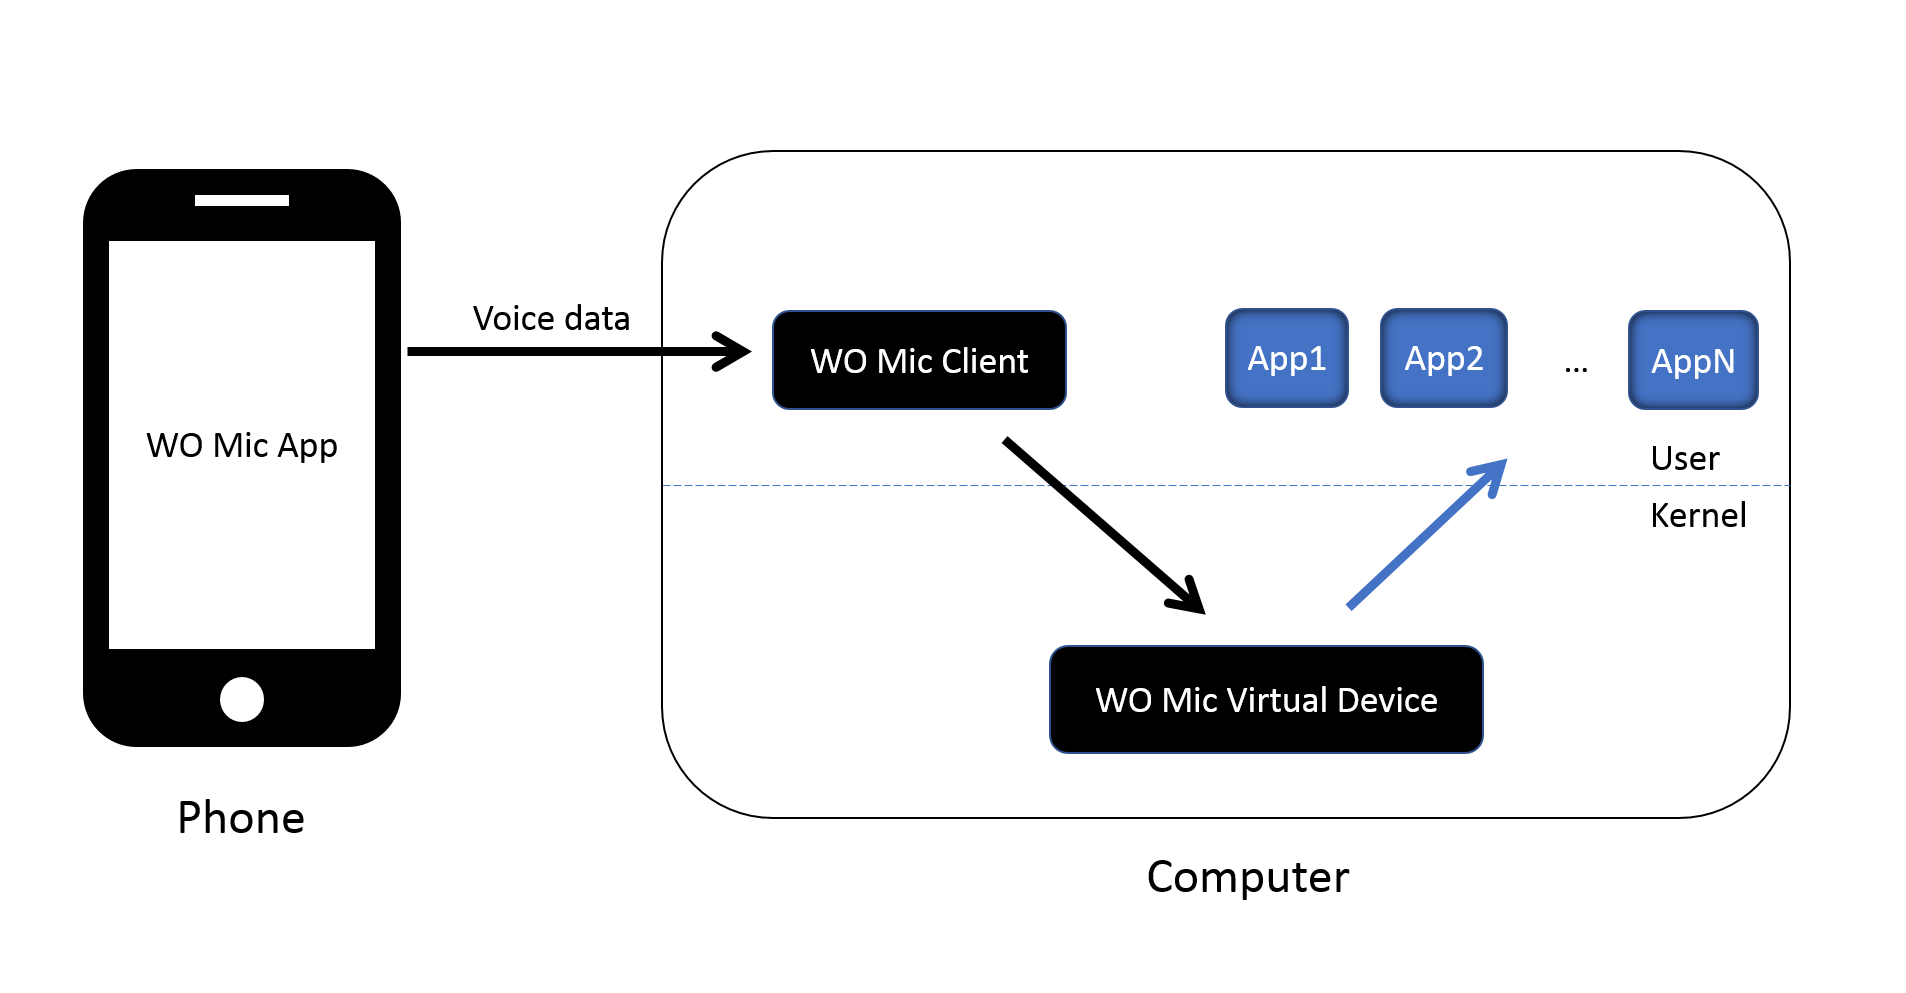
\includegraphics[width=0.65\textwidth]{Chapters/5CHP/Images/WOMICDiag.png}
    \caption{Flow of data in the components of the software}{\cite{WOMicFREE}}
    \label{fig:diagramWOMIC}
\end{figure}
In addition to this, is also necessary to install the drivers of the phone in use, if the connection is made over USB. To allow the access of the microphone in the PC, the transport mode must be selected on the phone application, USB in this case, in the app settings and after that start the application. In the PC the client software must be initialized and connected to the phone in the following order \textit{\>Connection\>Connect...} a new window will open, on which the USB must be selected as transport type and finalizing by pressing \textit{Connect}. With this, the microphone of the phone is available for use in the PC\cite{WOMicFREE}.
\section{Microcontroller}
%Introduction
%What is the purpose of each used element, Timer, UART, ADC, PINOUT for solenoid with timer
%What are the config of each
% Mainly from the ADC and how it works without having to use an additional timer
%
\subsection{Peripherals Configurations}
\subsubsection*{Timers}
In the configuration, two different timers were set, with the same configuration, one is used to measure the execution time of the algorithm and the other is used to set the amount of timer that the pin that triggers the solenoid is high. In this case were used Timer0\_A3 and Timer1\_A3, in both the counter mode of the timer is up, the division factor of the clock is 1 and they were set with a CCRx equal to 499, with this a interruption will occur at every 500$\mu$s.
\subsubsection*{ADC}
The LaunchPad in use offers ADC with a 10-bit, from the available pins, analog input 2 is selected. This input should be configured with the desire setting, to start is mandatory to disable the digital port of the pin to eliminate the flow of parasitic current flow, with the PySELx bits, by setting this bits HIGH it automatically enables the analog function of the port, although is still necessary to select the channel to conversion. The ADC will function in the sample and hold mode, using the timer from the ADC as the source of the sampling signal, the sample and hold period can be changed by software, to define the amount of clock cycles between each sample. 
\subsubsection*{eUSCI}
The eUSCI is used in UART mode to transfer data between the microcontroller and the PC, is used during the tests phase to perform two types of tests, one to test the algorithm and the other to receive data end send it to the PC. Both eUSCI\_A0 and eUSCI\_A1 support UART mode, unlike the eUSCI\_B0, the selected was the first, since works over the USB connection. In Transmission and Receiving, their were both set to work by polling with 115200bps of baud-rate, 8-bit, LSB first, no parity, no address and 1 stop bit.

\subsection{FFT implementation}
To process the signal captured from the ADC, is used a FFT algorithm. Two algorithms were considered to use in the microcontroller in use, a Fixed-Point and a Floating-Point versions, this algorithm was discovered by Cooley and Tukey in the beginning of the computer revolution and based on the complex DFT. The implementation used are based in FFT algorithm, and analysis the Fixed-Point and the Floating-Point side by side, they are quite similar, the main difference is in the data types used in each of the implementation, the fixed point can be adapted for the different types of signed integers, from 8-bits to 64-bits and uses a look-up table with the correspondent values of Sine and Cosine, used to calculate the real and imaginary in the frequency domain, this saves processing time, since isn't necessary to calculate these values while is the algorithm is running, on the other hand this limits the size of the vector to be processed, to be in maximum the size of the look-up table, unless the algorithm is adapted, this implementation is less time consuming for the microcontroller. The Floating-Point version calculates the values of the Sine and Cosine, and since it deals with values like float or double, which will require more memory and computational resources from the microcontroller if the same is used. Both implementation can be found on a repository in~\cite{262588213843476FixFft,Dannyf00FloatingPointFFTBenchmarka}, for a implementation from scratch there is also possible to find pseudo-code for that~\cite{smith1997scientist}.

The algorithms in use were adapted to fit in the purpose of the implementation for the microcontroller in use, as well as removed some option like the iFFT, which won't be necessary to use in this application.
\todo[inline,color=red!40]{Should I make a brief explanation of how the fft is implemented?}
After performing the FFT algorithm in the input data vector, is necessary to calculate the magnitude of the resulting data, since the algorithm returns complex values. To obtain the magnitude of the data in frequency is a simple mathematical operation and is described in~\ref{eq:magnitude}.
\begin{equation}\label{eq:magnitude}
    M = \sqrt{Re^2 + Im^2}
\end{equation}
\subsection{Fixed-Point Square Root}
For the application were the Fixed-Point is used is convenient to only deal with integers, after perform the FFT is necessary to calculate the magnitude of the signal, relative to the frequency, since the data returned from the algorithm is complex. For that as known, is necessary to use a the square root, several implementation of a Fixed-Point square root can be found, the implementation in use is an adaptation of the integer-to-integer version, from the repository~\cite{ChmikeFpsqrta}, in the used square root function, the input argument is a 32-bit value and the output a 16-bit value.

\section{MatLab}
This computational platform has various resources, with a lot appliances. For the purpose of the developed work only a few and simple function of this platform. In a initial stage, is going to be taken advantages of some of their function to generate random signals, in order to test the viability and precision of the FFT algorithm that will be used in a microcontroller environment, this requires the use of some basic mathematical functions and the serialport, the first is used to generate the random signal and the secondo to send the signal to to the microcontroller via UART, so it can be processed and the resulting data can be compared with the original. 

On other set of tests functions to record data from a certain audio input were used, to record the input of the microphone, each time that the LPG bottle is hit with the hammer. Beside this, the FFT function from the MATLAB is used to verify the response in frequency of the hit. 

Before the final application, is also need to verify the type of signals obtain in the sensors, after captured in the microcontroller the raw data is sent via UART to, once again, process them in the FFT function of MATLAB. 

\section{??}
% \begin{figure}[!htb]
%     \centering 
%         \begin{subfigure}[c]{\textwidth}
%             \centering
%             \input{Sections/3Transforms/Images/DFTSymmetry.tex}
%             \caption{}
%             \label{subfig:dft}
%         \end{subfigure}
%         \begin{subfigure}[c]{0.45\textwidth}
%             \centering
%             \input{Sections/3Transforms/Images/DCT1Symmetry.tex}
%             \caption{}
%             \label{subfig:dct1}
%         \end{subfigure}
%         \begin{subfigure}[c]{0.45\textwidth}
%             \centering
%             \input{Sections/3Transforms/Images/DCT2Symmetry.tex}
%             \caption{}
%             \label{subfig:dct2}
%         \end{subfigure}
%         \begin{subfigure}[c]{0.45\textwidth}
%             \centering
%             \input{Sections/3Transforms/Images/DCT3Symmetry.tex}
%             \caption{}
%             \label{subfig:dct3}
%         \end{subfigure}
%         \begin{subfigure}[c]{0.45\textwidth}
%             \centering
%             \input{Sections/3Transforms/Images/DCT4Symmetry.tex}
%             \caption{}
%             \label{subfig:dct4}
%         \end{subfigure}
%         \caption{Sequences generated in the first step of Table \ref{tab:DFTDCT}for the DFT and different DCTs. Filled dots correspond to the original sequence ((a) - \emph{DFT}; (b)) - \emph{DCT-I}; (c)) - \emph{DCT-II}; (d)) - \emph{DCT-III}; (e)) - \emph{DCT-IV}).}
%     \label{fig:2NSeq}
% \end{figure}
% \begin{lstlisting}
%     ./aomenc <INPUT-FILE> -h <HEIGHT> -w <WIDTH> -o <OUTPUT-FILE> --limit=10 -p 1 --cpu-used=8 --i420 --q-hist=64 --end-usage=q --cq-level=<CQ-LEVEL>
% \end{lstlisting}
%\addcontentsline{toc}{section}{References}
